      
               
                \begin{ledgroupsized}[r]{120mm}
                \footnotesize 
                \pstart                
                \noindent\textbf{\"{U}berlieferung:}   
                \pend
                \end{ledgroupsized}
            
              
                            \begin{ledgroupsized}[r]{114mm}
                            \footnotesize 
                            \pstart \parindent -6mm
                            \makebox[6mm][l]{\textit{L}}Konzept: LH XXXVII 5 Bl. 126. 1 Bl. 4\textsuperscript{o}. 1 S. R\"{u}ckseite leer.  Fig. 1 am oberen Rand links. Fig. 2 im oberen Drittel der Seite am linken Rand. Text umlaufend. In der Mitte des Blattes ein gut sichtbares Wasserzeichen.\\Cc 2 Nr. 964 B \pend
                            \end{ledgroupsized}
                %\normalsize
                \vspace*{5mm}
                \begin{ledgroup}
                \footnotesize 
                \pstart
            \noindent\footnotesize{\textbf{Datierungsgr\"{u}nde}: Von Leibniz datiert}
                \pend
                \end{ledgroup}
            
                \vspace*{8mm}
                \pstart 
                \normalsize
            [126~r\textsuperscript{o}] Maii 1675.  \pend \pstart \begin{wrapfigure}{l}{0.3\textwidth}                    
                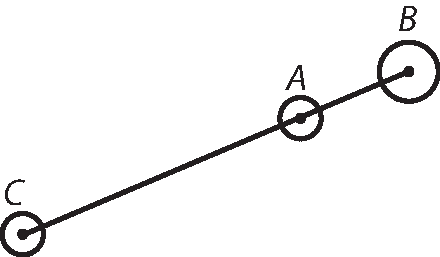
\includegraphics[width=0.3\textwidth]{images/lh03705126r-1}
              
                        %\caption{Bildbeschreibung}
                        \end{wrapfigure}
                       \textit{[Fig. 1]} \\
                    \noindent Les poids \textit{C}. \textit{B} estant en raison reciproque des distances   \textit{AC}, \textit{AB}. Il y aura equilibre, cela est,   bien connu par l'experience. Archim\`{e}de\protect\index{Namensregister}{\textso  {},} pretend de le demonstrer,\edtext{}{\lemma{demonstrer,}\Cfootnote{\textsc{Archimedes} von Syrakus, \cite{00317}\title{Planorum aequiponderantia, inventa, vel centra gravitatis planorum}, Basel 1544, S. 125f.}} il y avoit quelque chose \`{a} dire \`{a} la demonstration d'Archim\`{e}de\protect\index{Namensregister}{\textso  {},}, mais Mons. Huguens\protect\index{Namensregister}{\textso  {Huygens}, Christiaan (1629-1695)}  \`{a} ce qu'on dit l'a corrig\'{e}.\edtext{}{\lemma{corrig\'{e}.}\Cfootnote{vgl. dazu das Avertissement zu \textsc{Huygens},\cite{}\title{ Travaux divers de statique et de dynamique de 1659 \`{a} 1666}, in: \title{HO} XVI, S. 331 f.}} Galilaei\protect\index{Namensregister}{\textso  {Galilei}, Galileo (1564-1642)} et apres luy le Pere Pardies\protect\index{Namensregister}{\textso  {Pardies}, Ignace Gaston SJ (1636-1673)} avoient form\'{e} d'autres fa\c{c}ons   de raisonner.\edtext{}{\lemma{raisonner.}\Cfootnote{\textsc{G. Galilei}, \cite{00050}\title{Discorsi}, Leiden 1638, S. 109-111 (\title{GO} VIII, S. 152-154), I. G. \textsc{Pardies}, \cite{00296}\title{ La Statique}, Paris 1673, S. 33-40.}} Mais il me semble que tout cecy suppose ce qu'on appelle le centre de gravit\'{e}.   Au moins le P. Pardies\protect\index{Namensregister}{\textso {Pardies}, Ignace Gaston SJ (1636-1673} le suppose expr\`{e}s.  Sed quaecunque hujusmodi dicuntur de gravitatis centro supponunt legem naturae, quae efficiat, ut nihil agat  corpus, nisi lucretur. An falli possit natura, ut lucretur impraesentiarum,   plus autem perdat per consequentiam, (quod duarum virium complicatione \edtext{fieri forte potest}{\lemma{complicatione}\Bfootnote{ \textit{ (1) }\ an fieri possit \textit{ (2) }\ fieri forte potest \textit{ L }\ }}) alia quaestio est. Illud interea certum est, naturam   quo agit momento, lucrari.  \pend \pstart   \begin{center}                    
                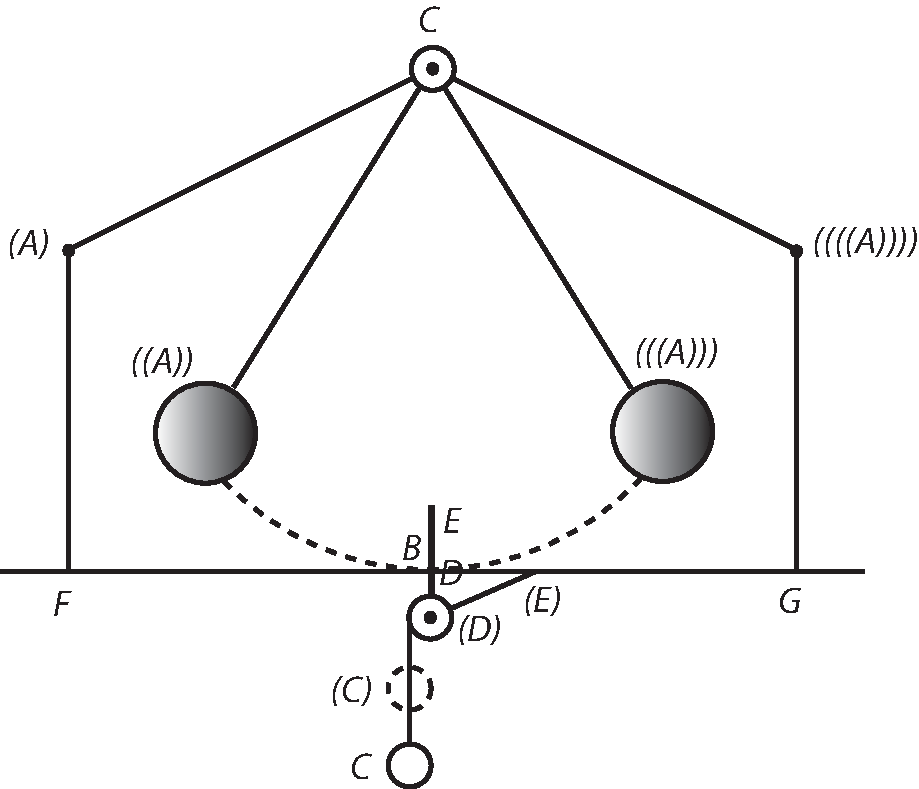
\includegraphics[width=0.8\textwidth]{images/lh03705126r-2}
              
                        %\caption{Bildbeschreibung}
                        \end{center}
                      \textit{[Fig. 1]}  \\
                     Sit pondus \textit{A} pendulum centro \textit{C}  quod ex puncto \textit{(A)} cadens per \textit{((A))}. \textit{B}. \textit{(((A)))} tandem perveniat in punctum \textit{((((A))))} in   itinere autem occurrens cuidam obstaculo in \textit{B}, quod sit \textit{DE}, idque abigens in \textit{(D)(E)} levet pondus \textit{C} in locum \textit{(C)}. Quo facilior sit calculus, vim omnem ponderis A,   reducamus in punctum, quod sit ejus centrum gravitatis  ejusque ponderis in punctum reducti vim, appellemus \textit{v}\edtext{. Ponatur}{\lemma{\textit{v.}}\Bfootnote{ \textit{ (1) }\ quo   in numerum impetuum seu in rectam AF, in cujus \textit{ (2) }\ . Ponatur \textit{ L }\ }} vis descensu \edtext{quaesita}{\lemma{quaesita}\Bfootnote{ \textit{ (1) }\ esse \textit{ (2) }\ componi \textit{ L }\ }} componi ex vi \textit{v} ducta in tempus \textit{t} quia quolibet temporis  momento nova vis impressa est, adeoque vis quaesita, seu percussionis vis, \textit{p} erit  \textit{vt}, seu $ap \sqcap vt.$  \pend \pstart Considerandum hic est aliquid, quod omiseram nempe non tantum eo motu elevari pondus \textit{C} in locum \textit{(C)} sed et altius elevari nonnihil, ipso   impetu ex duratione motus concepto. \pend \pstart  Et \edtext{ponendo}{\lemma{Et}\Bfootnote{ \textit{ (1) }\ in quantum \textit{ (2) }\ ponendo \textit{ L }\ }} pondus \textit{C} aequale ponderi F. necessario recta \textit{C(C)} erit differentia inter rectas   (A)F et ((((A))))G. Si vero sint inaequalia, erit \edtext{}{\lemma{}\Bfootnote{erit  \textbar\ pondus \textit{ gestr.}\ \textbar\ \textit{(A)F} \textit{ L }\ }} \textit{(A)F} - \textit{((((A))))G} ad  \textit{C(C)} reciproce ut pondus \textit{C} ad pondus \textit{A}. Nam si ope vectis aut Trochleae  connecti intelligantur \edtext{pondera \textit{(C)} et \textit{((((A))))} }{\lemma{intelligantur}\Bfootnote{ \textit{ (1) }\ puncta \textit{C} et \textit{ (2) }\ pondera \textit{(C)} et \textit{((((A))))}.  \textit{ L }\ }} patet tunc  descensu ponderis \textit{(C)} ad \textit{C} effici posse, ut elevetur \textit{((((A))))} donec fiat   aeque altum ipsi \textit{(A)}.  \pend \pstart   Sed ex his nondum scitur \edtext{dato  pondere \textit{AF}, et tempore lapsus, et recta [\textit{(A)F}]\edtext{}{\Bfootnote{\textit{AF}\textit{\ L \"{a}ndert Hrsg. } }}, seu lapsus altitudine}{\lemma{scitur}\Bfootnote{ \textit{ (1) }\ data celeritate ponderis \textit{ (2) }\ data vi et altitudine  \textit{(a)}\ po \textit{(b)}\ lapsus \textit{ (3) }\ dato [ ... ] altitudine \textit{ L }\ }}, datoque pondere \textit{C}   quanta debeat esse recta \textit{C(C)} et quantum tempus quo percurritur.  \pend \pstart   Si non pondus elevandum, sed elaterium tendendum sit, eodem res modo aestimanda   est, nimirum elaterii illius tensioni aequabitur elevatio ponderis tanta, in quantam   disploso elaterio ponderis attolli potest. Et hoc aestimationis modo poterimus \edtext{Elateria ponderibus aequiparare}{\lemma{poterimus}\Bfootnote{ \textit{ (1) }\ definire \textit{ (2) }\ Elateria ponderibus aequiparare \textit{ L }\ }}, et Centra gravitatis hic quoque   concipere.  \pend \pstart   Si in figura nostra celeri motu transeat pondus \textit{A} \edtext{}{\lemma{}\Bfootnote{A.  \textbar\ ipse \textit{ gestr.}\ \textbar\ pondus \textit{ L }\ }} pondus \textit{C} pauco tempore   elevabit ad magnam altitudinem, ideoque ut fit pendulo assurgente, parum etiam ictus ipsi   infligetur, quia ictus temporibus aestimandi sunt. \pend \pstart  Sed contra non videtur ictus temporibus aestimandos, alioqui, corpora celerius ascendentia, non ideo plures acciperent ictus   contrarios. Itaque exacte loquendo considerandus ictuum numerus, et quantitas, quantitas tum a magnitudine corpus, tum a gradu celeritatis aestimatur.  \pend 
 


 


 


 


 

